\section{\hspace{1em} Числени симулации}

\subsection{Използвани параметри и софтуер}
Представените симулации използват параметри от таблица \ref{tbl:ParameterValues}. \\
За генериране на различни набори от параметри, общо изследване на траектории и генериране на данни за равновесните точки и решения на системата \eqref{eq:TheDimensionlessProblem} е използвана компютърната система \texttt{Mathematica}. \\
% Кодът за намирането на ядрото на слаба инвариантност на Белман за едномерната форма на модела, т.е. \eqref{eq:RepellentProblem} беше получен от доцент Петър Рашков (ръководител на дипломната работа и написал статията \cite{Rashkov2022} за \eqref{eq:RepellentProblem}) на \texttt{MATLAB} и след малки промени изпълняван на \texttt{Octave}, като след това беше преведен на \texttt{C++}.
За решаване на задачата \eqref{eq:ViabilityKernel} чрез формулировката \eqref{eq:HJBTime} е направена имплементация на \texttt{C++}, като не се били нужни библиотеки освен стандартната \texttt{std}. \\
Графиките на (проекциите на) решенията на \eqref{eq:TheDimensionlessProblem} и heat-map на равновесните точки са получени чрез \texttt{gnuplot}. \\
За изчисление на стойностите в таблицата \ref{tbl:ViabilityKernel-poster} е ползван софтуерът за електронни таблици (spreadsheet) \texttt{LibreOffice Calc}. \\
Кодът може да бъде намерен на адрес \url{https://github.com/kaloan/master-thesis/tree/master/code}.

\begin{remark}
  Поради кооперативността на \eqref{eq:TheDimensionlessProblem} представените симулации са за $\mathbf{u}(t) \equiv \bar{\mathbf{u}}$, тъй като ако може системата да бъде управлявана спрямо здравната политика с някаква по-малка употреба на репелент, може и с максималната.
  Така ако не се управлява с максималната, не може с никаква.
  Поради характера на задачата е възможно в някои случаи да няма единствено управление, което да удовлетворява зададените от здравната политика ограничения.
  В такива случаи за намиране на други възможни $\mathbf{u}(t)$ могат да се използват методи от \cite{Assellaou2016, Assellaou2018}.
\end{remark}

\begin{table}[H]
  \centering
  \begin{tabular}{ |c ||c c c c c c|  }
    % \hhline{~------}
    \hline
    \multirow{2}{*}{Параметър}& \multicolumn{2}{c}{Набор 1}& \multicolumn{2}{c}{Набор 2} & \multicolumn{2}{c|}{Набор 3}\\
    & М. 1 & М. 2 & М. 1 & М. 2 & М. 1 & М. 2\\
    \hline
    % \hhline{~------}
    $\beta_{vh}$ & \multicolumn{2}{c}{$0.5$} & \multicolumn{2}{c}{$0.5$}  & \multicolumn{2}{c|}{$0.5$}\\
    $\beta_{hv}$ & \multicolumn{2}{c}{$0.1$} & \multicolumn{2}{c}{$0.1$} & \multicolumn{2}{c|}{$0.1$}\\
    $a_i$ & $0.12$ & $0.18$ & $0.158$ & $0.159$ & $0.15$ & $0.24$\\
    $M_i$ & $6 \times 10^7$ & $1.6 \times 10^8$ & $7320950$ & $4695340$ & $7320950$ & $4695340$\\
    $\mu_i$ & $\frac{1}{21}$ & $\frac{1}{15}$ & $0.032$ & $0.046$ & $0.0397$ & $0.0335$\\
    $\tau$ & \multicolumn{2}{c}{$10$} & \multicolumn{2}{c}{$10$} & \multicolumn{2}{c|}{$10$}\\
    $N_i$ & $8 \times 10^6$ & $2 \times 10^7$ & $9377980$ & $4467650$ & $755440$ & $3945290$\\
    $\gamma_i$ & \multicolumn{2}{c}{$\frac{1}{14}$} & $0.0627$ & $0.0576$ & $0.0735$ & $0.0622$\\
    $p_{ij}$ & \multicolumn{6}{c|}{различни ($p_{i1}+p_{i2}=1$)}\\
    $\kappa$ & \multicolumn{2}{c}{$0.44$} & \multicolumn{2}{c}{$0.37$} & \multicolumn{2}{c|}{$0.38$}\\
    $\bar{u}_i$ & $0.15$ & $0.3$ & $0.39$ & $0.12$ & $0.35$ & $0.3$\\
    $\bar{I}_i$ & $0.1$ & $0.14$ & $0.065$ & $0.12$ & $0.09$ & $0.09$\\
    \hline
  \end{tabular}
  \caption{Таблица със стойностите на параметрите от таблица \ref{tbl:ParameterDefinitions} за числени симулации}
  \label{tbl:ParameterValues}
\end{table}

\subsection{Равновесни точки спрямо $\bar{\mathbf{u}}$}

След направени редица числени експерименти чрез произволен набор (но рамките на физически значимите) от параметри се забеляза, че ендемичните точки са често силно променливи спрямо мобилността и то (в общия случай) по нелинеен начин (фигури \ref{fig:EquilibriumPoints-poster}, \ref{fig:EquilibriumPoints-03-19-16-12-04} и \ref{fig:EquilibriumPoints-03-19-16-58-19}). Ето някои бележки за ендемичните състояния:
\begin{enumerate}
  \item Възможно е в двете местообитания да липсва ендемизъм за произволен избор на мобилности (няма фигура, но очевидно лесно се достига за малки $a_i$ и големи $\bar{u}_i, \kappa$).
    %\item Възможно е в едното местообитание да липсва ендемизъм при всевъзможните мобилности, но в другото поне за някои от тях да има.
  \item Възможно е при промяна само на мобилността на жителите за едното местообитание да получим различно ендемично състояние. Най-интересният пример за това е фигура \ref{fig:EquilibriumPoints-03-19-16-12-04}, където $x_1^*$ се изменя първо растейки, а после намалявайки при намаляване на $p_{11}$ (т.е. увеличавайки движението на жителите на първото към второто).
  \item Възможно е между два избора на мобилности в едното местообетание да няма съществена разлика в пропорцията на ендемично заразени, но за другото да има (фигура \ref{fig:EquilibriumPoints-03-19-16-58-19}).
  \item Често в областта на малки мобилности $p_{11}, p_{22} \approx 1$ има силно изменение в пропорцията заразени в ендемичното състояние (фигури \ref{fig:EquilibriumPoints-03-19-16-12-04} и \ref{fig:EquilibriumPoints-03-19-16-58-19}).
\end{enumerate}

\begin{figure}[H]
  \centering
  \includegraphics{equilibrium-poster.pdf}
  \caption{Равновесните точки на \eqref{eq:TheDimensionlessProblem}} с параметрите от набор 1 от таблица \ref{tbl:ParameterValues}
  \label{fig:EquilibriumPoints-poster}
\end{figure}
% % GNUPLOT: LaTeX picture with Postscript
\documentclass{minimal}
% Set font size
\makeatletter
\def\@ptsize{0}
\InputIfFileExists{size10.clo}{}{%
   \GenericError{(gnuplot) \space\space\space\@spaces}{%
      Gnuplot Error: File `size10.clo' not found! Could not set font size%
   }{See the gnuplot documentation for explanation.%
   }{For using a font size a file `size<fontsize>.clo' has to exist.
        Falling back ^^Jto default fontsize 10pt.}%
  \def\@ptsize{0}
  \input{size10.clo}%
}%
\makeatother
% Load packages
\usepackage{calc}
\usepackage{graphicx}
\usepackage{color}
\makeatletter
% Select an appropriate default driver (from TeXLive graphics.cfg)
\begingroup
  \chardef\x=0 %
  % check pdfTeX
  \@ifundefined{pdfoutput}{}{%
    \ifcase\pdfoutput
    \else
      \chardef\x=1 %
    \fi
  }%
  % check VTeX
  \@ifundefined{OpMode}{}{%
    \chardef\x=2 %
  }%
\expandafter\endgroup
\ifcase\x
  % default case
  \PassOptionsToPackage{dvips}{geometry}
\or
  % pdfTeX is running in pdf mode
  \PassOptionsToPackage{pdftex}{geometry}
\else
  % VTeX is running
  \PassOptionsToPackage{vtex}{geometry}
\fi
\makeatother
% Set papersize
\usepackage[papersize={374.40bp,172.80bp},text={374.40bp,172.80bp}]{geometry}
% No page numbers and no paragraph indentation
\pagestyle{empty}
\setlength{\parindent}{0bp}%
% Load configuration file
\InputIfFileExists{gnuplot.cfg}{%
  \typeout{Using configuration file gnuplot.cfg}%
}{%
 \typeout{No configuration file gnuplot.cfg found.}%
}%
%
\begin{document}
\begingroup
  \makeatletter
  \providecommand\color[2][]{%
    \GenericError{(gnuplot) \space\space\space\@spaces}{%
      Package color not loaded in conjunction with
      terminal option `colourtext'%
    }{See the gnuplot documentation for explanation.%
    }{Either use 'blacktext' in gnuplot or load the package
      color.sty in LaTeX.}%
    \renewcommand\color[2][]{}%
  }%
  \providecommand\includegraphics[2][]{%
    \GenericError{(gnuplot) \space\space\space\@spaces}{%
      Package graphicx or graphics not loaded%
    }{See the gnuplot documentation for explanation.%
    }{The gnuplot epslatex terminal needs graphicx.sty or graphics.sty.}%
    \renewcommand\includegraphics[2][]{}%
  }%
  \providecommand\rotatebox[2]{#2}%
  \@ifundefined{ifGPcolor}{%
    \newif\ifGPcolor
    \GPcolortrue
  }{}%
  \@ifundefined{ifGPblacktext}{%
    \newif\ifGPblacktext
    \GPblacktexttrue
  }{}%
  % define a \g@addto@macro without @ in the name:
  \let\gplgaddtomacro\g@addto@macro
  % define empty templates for all commands taking text:
  \gdef\gplbacktext{}%
  \gdef\gplfronttext{}%
  \makeatother
  \ifGPblacktext
    % no textcolor at all
    \def\colorrgb#1{}%
    \def\colorgray#1{}%
  \else
    % gray or color?
    \ifGPcolor
      \def\colorrgb#1{\color[rgb]{#1}}%
      \def\colorgray#1{\color[gray]{#1}}%
      \expandafter\def\csname LTw\endcsname{\color{white}}%
      \expandafter\def\csname LTb\endcsname{\color{black}}%
      \expandafter\def\csname LTa\endcsname{\color{black}}%
      \expandafter\def\csname LT0\endcsname{\color[rgb]{1,0,0}}%
      \expandafter\def\csname LT1\endcsname{\color[rgb]{0,1,0}}%
      \expandafter\def\csname LT2\endcsname{\color[rgb]{0,0,1}}%
      \expandafter\def\csname LT3\endcsname{\color[rgb]{1,0,1}}%
      \expandafter\def\csname LT4\endcsname{\color[rgb]{0,1,1}}%
      \expandafter\def\csname LT5\endcsname{\color[rgb]{1,1,0}}%
      \expandafter\def\csname LT6\endcsname{\color[rgb]{0,0,0}}%
      \expandafter\def\csname LT7\endcsname{\color[rgb]{1,0.3,0}}%
      \expandafter\def\csname LT8\endcsname{\color[rgb]{0.5,0.5,0.5}}%
    \else
      % gray
      \def\colorrgb#1{\color{black}}%
      \def\colorgray#1{\color[gray]{#1}}%
      \expandafter\def\csname LTw\endcsname{\color{white}}%
      \expandafter\def\csname LTb\endcsname{\color{black}}%
      \expandafter\def\csname LTa\endcsname{\color{black}}%
      \expandafter\def\csname LT0\endcsname{\color{black}}%
      \expandafter\def\csname LT1\endcsname{\color{black}}%
      \expandafter\def\csname LT2\endcsname{\color{black}}%
      \expandafter\def\csname LT3\endcsname{\color{black}}%
      \expandafter\def\csname LT4\endcsname{\color{black}}%
      \expandafter\def\csname LT5\endcsname{\color{black}}%
      \expandafter\def\csname LT6\endcsname{\color{black}}%
      \expandafter\def\csname LT7\endcsname{\color{black}}%
      \expandafter\def\csname LT8\endcsname{\color{black}}%
    \fi
  \fi
    \setlength{\unitlength}{0.0500bp}%
    \ifx\gptboxheight\undefined%
      \newlength{\gptboxheight}%
      \newlength{\gptboxwidth}%
      \newsavebox{\gptboxtext}%
    \fi%
    \setlength{\fboxrule}{0.5pt}%
    \setlength{\fboxsep}{1pt}%
    \definecolor{tbcol}{rgb}{1,1,1}%
\begin{picture}(7488.00,3456.00)%
    \gplgaddtomacro\gplbacktext{%
      \csname LTb\endcsname%%
      \put(860,912){\makebox(0,0)[r]{\strut{}$0.8$}}%
      \put(860,1346){\makebox(0,0)[r]{\strut{}$0.85$}}%
      \put(860,1779){\makebox(0,0)[r]{\strut{}$0.9$}}%
      \put(860,2213){\makebox(0,0)[r]{\strut{}$0.95$}}%
      \put(860,2646){\makebox(0,0)[r]{\strut{}$1$}}%
      \put(1043,649){\makebox(0,0){\strut{}$0.8$}}%
      \put(1477,649){\makebox(0,0){\strut{}$0.85$}}%
      \put(1910,649){\makebox(0,0){\strut{}$0.9$}}%
      \put(2344,649){\makebox(0,0){\strut{}$0.95$}}%
      \put(2777,649){\makebox(0,0){\strut{}$1$}}%
    }%
    \gplgaddtomacro\gplfronttext{%
      \csname LTb\endcsname%%
      \put(190,1779){\rotatebox{-270.00}{\makebox(0,0){\strut{}$p_{22}$}}}%
      \put(1910,349){\makebox(0,0){\strut{}$p_{11}$}}%
      \put(3026,912){\makebox(0,0)[l]{\strut{}$0$}}%
      \put(3026,1258){\makebox(0,0)[l]{\strut{}$0.005$}}%
      \put(3026,1605){\makebox(0,0)[l]{\strut{}$0.01$}}%
      \put(3026,1952){\makebox(0,0)[l]{\strut{}$0.015$}}%
      \put(3026,2299){\makebox(0,0)[l]{\strut{}$0.02$}}%
      \put(3026,2646){\makebox(0,0)[l]{\strut{}$0.025$}}%
      \put(1910,2946){\makebox(0,0){\strut{}$X_1^*$}}%
    }%
    \gplgaddtomacro\gplbacktext{%
      \csname LTb\endcsname%%
      \put(4604,912){\makebox(0,0)[r]{\strut{}$0.8$}}%
      \put(4604,1346){\makebox(0,0)[r]{\strut{}$0.85$}}%
      \put(4604,1779){\makebox(0,0)[r]{\strut{}$0.9$}}%
      \put(4604,2213){\makebox(0,0)[r]{\strut{}$0.95$}}%
      \put(4604,2646){\makebox(0,0)[r]{\strut{}$1$}}%
      \put(4787,649){\makebox(0,0){\strut{}$0.8$}}%
      \put(5221,649){\makebox(0,0){\strut{}$0.85$}}%
      \put(5654,649){\makebox(0,0){\strut{}$0.9$}}%
      \put(6088,649){\makebox(0,0){\strut{}$0.95$}}%
      \put(6521,649){\makebox(0,0){\strut{}$1$}}%
    }%
    \gplgaddtomacro\gplfronttext{%
      \csname LTb\endcsname%%
      \put(3934,1779){\rotatebox{-270.00}{\makebox(0,0){\strut{}$p_{22}$}}}%
      \put(5654,349){\makebox(0,0){\strut{}$p_{11}$}}%
      \put(6770,912){\makebox(0,0)[l]{\strut{}$0$}}%
      \put(6770,1128){\makebox(0,0)[l]{\strut{}$0.01$}}%
      \put(6770,1345){\makebox(0,0)[l]{\strut{}$0.02$}}%
      \put(6770,1562){\makebox(0,0)[l]{\strut{}$0.03$}}%
      \put(6770,1779){\makebox(0,0)[l]{\strut{}$0.04$}}%
      \put(6770,1995){\makebox(0,0)[l]{\strut{}$0.05$}}%
      \put(6770,2212){\makebox(0,0)[l]{\strut{}$0.06$}}%
      \put(6770,2429){\makebox(0,0)[l]{\strut{}$0.07$}}%
      \put(6770,2646){\makebox(0,0)[l]{\strut{}$0.08$}}%
      \put(5654,2946){\makebox(0,0){\strut{}$X_2^*$}}%
    }%
    \gplbacktext
    \put(0,0){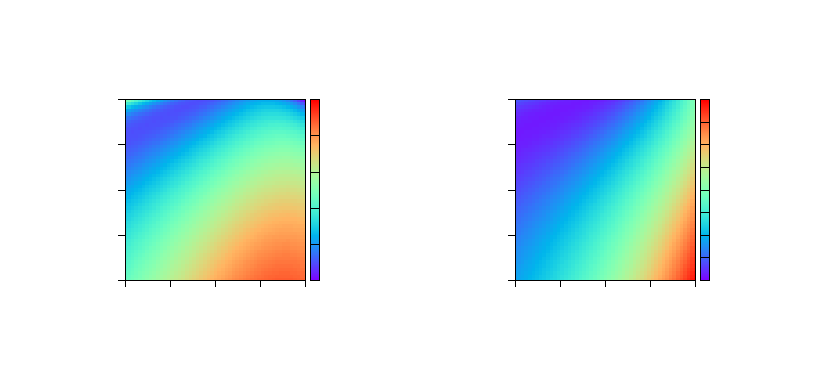
\includegraphics[width={374.40bp},height={172.80bp}]{equilibrium1-inc}}%
    \gplfronttext
  \end{picture}%
\endgroup
\end{document}


\begin{figure}[H]
  \centering
  \includegraphics{equilibrium-03-19-16-12-04.pdf}
  \caption{Равновесните точки на \eqref{eq:TheDimensionlessProblem}} с параметрите от набор 2 от таблица \ref{tbl:ParameterValues}
  \label{fig:EquilibriumPoints-03-19-16-12-04}
\end{figure}
% % GNUPLOT: LaTeX picture with Postscript
\documentclass{minimal}
% Set font size
\makeatletter
\def\@ptsize{0}
\InputIfFileExists{size10.clo}{}{%
   \GenericError{(gnuplot) \space\space\space\@spaces}{%
      Gnuplot Error: File `size10.clo' not found! Could not set font size%
   }{See the gnuplot documentation for explanation.%
   }{For using a font size a file `size<fontsize>.clo' has to exist.
        Falling back ^^Jto default fontsize 10pt.}%
  \def\@ptsize{0}
  \input{size10.clo}%
}%
\makeatother
% Load packages
\usepackage{calc}
\usepackage{graphicx}
\usepackage{color}
\makeatletter
% Select an appropriate default driver (from TeXLive graphics.cfg)
\begingroup
  \chardef\x=0 %
  % check pdfTeX
  \@ifundefined{pdfoutput}{}{%
    \ifcase\pdfoutput
    \else
      \chardef\x=1 %
    \fi
  }%
  % check VTeX
  \@ifundefined{OpMode}{}{%
    \chardef\x=2 %
  }%
\expandafter\endgroup
\ifcase\x
  % default case
  \PassOptionsToPackage{dvips}{geometry}
\or
  % pdfTeX is running in pdf mode
  \PassOptionsToPackage{pdftex}{geometry}
\else
  % VTeX is running
  \PassOptionsToPackage{vtex}{geometry}
\fi
\makeatother
% Set papersize
\usepackage[papersize={374.40bp,172.80bp},text={374.40bp,172.80bp}]{geometry}
% No page numbers and no paragraph indentation
\pagestyle{empty}
\setlength{\parindent}{0bp}%
% Load configuration file
\InputIfFileExists{gnuplot.cfg}{%
  \typeout{Using configuration file gnuplot.cfg}%
}{%
 \typeout{No configuration file gnuplot.cfg found.}%
}%
%
\begin{document}
\begingroup
  \makeatletter
  \providecommand\color[2][]{%
    \GenericError{(gnuplot) \space\space\space\@spaces}{%
      Package color not loaded in conjunction with
      terminal option `colourtext'%
    }{See the gnuplot documentation for explanation.%
    }{Either use 'blacktext' in gnuplot or load the package
      color.sty in LaTeX.}%
    \renewcommand\color[2][]{}%
  }%
  \providecommand\includegraphics[2][]{%
    \GenericError{(gnuplot) \space\space\space\@spaces}{%
      Package graphicx or graphics not loaded%
    }{See the gnuplot documentation for explanation.%
    }{The gnuplot epslatex terminal needs graphicx.sty or graphics.sty.}%
    \renewcommand\includegraphics[2][]{}%
  }%
  \providecommand\rotatebox[2]{#2}%
  \@ifundefined{ifGPcolor}{%
    \newif\ifGPcolor
    \GPcolortrue
  }{}%
  \@ifundefined{ifGPblacktext}{%
    \newif\ifGPblacktext
    \GPblacktexttrue
  }{}%
  % define a \g@addto@macro without @ in the name:
  \let\gplgaddtomacro\g@addto@macro
  % define empty templates for all commands taking text:
  \gdef\gplbacktext{}%
  \gdef\gplfronttext{}%
  \makeatother
  \ifGPblacktext
    % no textcolor at all
    \def\colorrgb#1{}%
    \def\colorgray#1{}%
  \else
    % gray or color?
    \ifGPcolor
      \def\colorrgb#1{\color[rgb]{#1}}%
      \def\colorgray#1{\color[gray]{#1}}%
      \expandafter\def\csname LTw\endcsname{\color{white}}%
      \expandafter\def\csname LTb\endcsname{\color{black}}%
      \expandafter\def\csname LTa\endcsname{\color{black}}%
      \expandafter\def\csname LT0\endcsname{\color[rgb]{1,0,0}}%
      \expandafter\def\csname LT1\endcsname{\color[rgb]{0,1,0}}%
      \expandafter\def\csname LT2\endcsname{\color[rgb]{0,0,1}}%
      \expandafter\def\csname LT3\endcsname{\color[rgb]{1,0,1}}%
      \expandafter\def\csname LT4\endcsname{\color[rgb]{0,1,1}}%
      \expandafter\def\csname LT5\endcsname{\color[rgb]{1,1,0}}%
      \expandafter\def\csname LT6\endcsname{\color[rgb]{0,0,0}}%
      \expandafter\def\csname LT7\endcsname{\color[rgb]{1,0.3,0}}%
      \expandafter\def\csname LT8\endcsname{\color[rgb]{0.5,0.5,0.5}}%
    \else
      % gray
      \def\colorrgb#1{\color{black}}%
      \def\colorgray#1{\color[gray]{#1}}%
      \expandafter\def\csname LTw\endcsname{\color{white}}%
      \expandafter\def\csname LTb\endcsname{\color{black}}%
      \expandafter\def\csname LTa\endcsname{\color{black}}%
      \expandafter\def\csname LT0\endcsname{\color{black}}%
      \expandafter\def\csname LT1\endcsname{\color{black}}%
      \expandafter\def\csname LT2\endcsname{\color{black}}%
      \expandafter\def\csname LT3\endcsname{\color{black}}%
      \expandafter\def\csname LT4\endcsname{\color{black}}%
      \expandafter\def\csname LT5\endcsname{\color{black}}%
      \expandafter\def\csname LT6\endcsname{\color{black}}%
      \expandafter\def\csname LT7\endcsname{\color{black}}%
      \expandafter\def\csname LT8\endcsname{\color{black}}%
    \fi
  \fi
    \setlength{\unitlength}{0.0500bp}%
    \ifx\gptboxheight\undefined%
      \newlength{\gptboxheight}%
      \newlength{\gptboxwidth}%
      \newsavebox{\gptboxtext}%
    \fi%
    \setlength{\fboxrule}{0.5pt}%
    \setlength{\fboxsep}{1pt}%
    \definecolor{tbcol}{rgb}{1,1,1}%
\begin{picture}(7488.00,3456.00)%
    \gplgaddtomacro\gplbacktext{%
      \csname LTb\endcsname%%
      \put(860,912){\makebox(0,0)[r]{\strut{}$0.8$}}%
      \put(860,1346){\makebox(0,0)[r]{\strut{}$0.85$}}%
      \put(860,1779){\makebox(0,0)[r]{\strut{}$0.9$}}%
      \put(860,2213){\makebox(0,0)[r]{\strut{}$0.95$}}%
      \put(860,2646){\makebox(0,0)[r]{\strut{}$1$}}%
      \put(1043,649){\makebox(0,0){\strut{}$0.8$}}%
      \put(1477,649){\makebox(0,0){\strut{}$0.85$}}%
      \put(1910,649){\makebox(0,0){\strut{}$0.9$}}%
      \put(2344,649){\makebox(0,0){\strut{}$0.95$}}%
      \put(2777,649){\makebox(0,0){\strut{}$1$}}%
    }%
    \gplgaddtomacro\gplfronttext{%
      \csname LTb\endcsname%%
      \put(190,1779){\rotatebox{-270.00}{\makebox(0,0){\strut{}$p_{22}$}}}%
      \put(1910,349){\makebox(0,0){\strut{}$p_{11}$}}%
      \put(3026,912){\makebox(0,0)[l]{\strut{}$0$}}%
      \put(3026,1258){\makebox(0,0)[l]{\strut{}$0.005$}}%
      \put(3026,1605){\makebox(0,0)[l]{\strut{}$0.01$}}%
      \put(3026,1952){\makebox(0,0)[l]{\strut{}$0.015$}}%
      \put(3026,2299){\makebox(0,0)[l]{\strut{}$0.02$}}%
      \put(3026,2646){\makebox(0,0)[l]{\strut{}$0.025$}}%
      \put(1910,2946){\makebox(0,0){\strut{}$X_1^*$}}%
    }%
    \gplgaddtomacro\gplbacktext{%
      \csname LTb\endcsname%%
      \put(4604,912){\makebox(0,0)[r]{\strut{}$0.8$}}%
      \put(4604,1346){\makebox(0,0)[r]{\strut{}$0.85$}}%
      \put(4604,1779){\makebox(0,0)[r]{\strut{}$0.9$}}%
      \put(4604,2213){\makebox(0,0)[r]{\strut{}$0.95$}}%
      \put(4604,2646){\makebox(0,0)[r]{\strut{}$1$}}%
      \put(4787,649){\makebox(0,0){\strut{}$0.8$}}%
      \put(5221,649){\makebox(0,0){\strut{}$0.85$}}%
      \put(5654,649){\makebox(0,0){\strut{}$0.9$}}%
      \put(6088,649){\makebox(0,0){\strut{}$0.95$}}%
      \put(6521,649){\makebox(0,0){\strut{}$1$}}%
    }%
    \gplgaddtomacro\gplfronttext{%
      \csname LTb\endcsname%%
      \put(3934,1779){\rotatebox{-270.00}{\makebox(0,0){\strut{}$p_{22}$}}}%
      \put(5654,349){\makebox(0,0){\strut{}$p_{11}$}}%
      \put(6770,912){\makebox(0,0)[l]{\strut{}$0$}}%
      \put(6770,1128){\makebox(0,0)[l]{\strut{}$0.01$}}%
      \put(6770,1345){\makebox(0,0)[l]{\strut{}$0.02$}}%
      \put(6770,1562){\makebox(0,0)[l]{\strut{}$0.03$}}%
      \put(6770,1779){\makebox(0,0)[l]{\strut{}$0.04$}}%
      \put(6770,1995){\makebox(0,0)[l]{\strut{}$0.05$}}%
      \put(6770,2212){\makebox(0,0)[l]{\strut{}$0.06$}}%
      \put(6770,2429){\makebox(0,0)[l]{\strut{}$0.07$}}%
      \put(6770,2646){\makebox(0,0)[l]{\strut{}$0.08$}}%
      \put(5654,2946){\makebox(0,0){\strut{}$X_2^*$}}%
    }%
    \gplbacktext
    \put(0,0){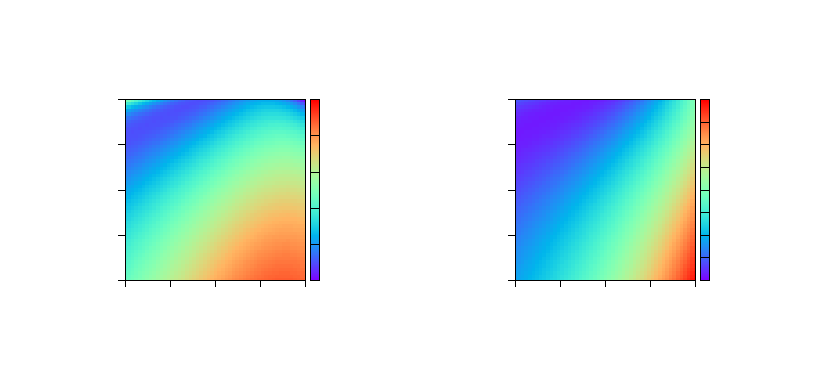
\includegraphics[width={374.40bp},height={172.80bp}]{equilibrium1-inc}}%
    \gplfronttext
  \end{picture}%
\endgroup
\end{document}


\begin{figure}[H]
  \centering
  \includegraphics{equilibrium-03-19-16-58-19.pdf}
  \caption{Равновесните точки на \eqref{eq:TheDimensionlessProblem}} с параметрите от набор 3 от таблица \ref{tbl:ParameterValues}
  \label{fig:EquilibriumPoints-03-19-16-58-19}
\end{figure}

\subsection{Графики на решението}
Във фигура \ref{fig:Solution-poster} може да се забележат няколко особености.
Ако се разглеждат местообитанията независимо, то ако не се използва репелент в първото местообитание има ендемично състояние, а ако се използва репелент, то отсъства.
Също така в двата случая не се спазва здравната политика на първото местообитание за 2-3 месеца.
Ако вече е налична мобилност, но без употреба на репелент, то от това че ендемичното състояние $x_1^*$ е над тавана на заразени $\bar{I}_1$ не се спазва здравната политика за произволно дълъг период.
Ако има и мобилност, и употреба на репелент, то здравната политика се спазва, но все пак заболяването има ендемичен характер.
В местообитание 2 няма голяма разлика между това дали има или няма мобилност, но при мобилност пика на заразени е по-голям в местообитание 2 отколкото без. Високият таван на заразени $\bar{I}_2$ явно действа като буфер за заразени от местообитание 1.

\begin{figure}[H]
  \centering
  \includegraphics{solution-poster.pdf}
  \caption{Решението на \eqref{eq:TheDimensionlessProblem} с параметрите от набор 1 таблица \ref{tbl:ParameterValues} и $\mathbf{z}_0=(0.0572, 0.048, 0.052, 0.044)^T$.\\
    Пунктирано: без употреба на репелент ($\mathbf{u}(t) \equiv \mathbf{0}$), плътно: максимална употреба на репелент ($\mathbf{u}(t) \equiv \bar{\mathbf{u}}$).\\
  Червено: без мобилност ($p_{11}=p_{22}=1$), синьо: с мобилност ($p_{11}=p_{22}=0.85$)}
  \label{fig:Solution-poster}
\end{figure}

Същото начално условие за фигура \ref{fig:Solution-poster} е взето и за фигура \ref{fig:Solution-03-19-16-12-04}.
Очевидно то не е от $V(\bar{\mathbf{I}}, \bar{\mathbf{u}})$, защото не се спазва здравната политика на местообитание 2 дори при максимална употреба на репелент.
Вижда се, че няма голяма разлика в поведението на заразата спрямо мобилността и употребата на репелент в местообитание 2.
От друга страна случаят с местообитание 1 е интересен.
Стига да няма мобилност, дори и без употреба на репелент липсва ендемизъм, като за 2-3 седмици едвам не се изпълнява здравната политика, а когато се използва, то е изпълнена за целия период.
Когато присъства мобилност, то без репелент отново за 2-3 седмици едвам не се изпълнява здравната политика, но пък сега вече присъства ендемизъм $x_1^* \approx \bar{I}_1$.
Също така има 2-3 месеца, в които броят заразени се понижава, преди пак да се увеличи.
При мобилност и с репелент отново заболяването има ендемичен характер, но винаги се спазва здравната политика и вече $x_1^* \approx \frac{1}{2}\bar{I}_1$.

\begin{figure}[H]
  \centering
  \includegraphics{solution-03-19-16-12-04.pdf}
  \caption{Решението на \eqref{eq:TheDimensionlessProblem} с параметрите от набор 2 от таблица \ref{tbl:ParameterValues} и $\mathbf{z}_0=(0.0572, 0.048, 0.052, 0.044)^T$.\\
    Пунктирано: без употреба на репелент ($\mathbf{u}(t) \equiv \mathbf{0}$), плътно: максимална употреба на репелент ($\mathbf{u}(t) \equiv \bar{\mathbf{u}}$).\\
  Червено: без мобилност ($p_{11}=p_{22}=1$), синьо: с мобилност ($p_{11}=0.99, p_{22}=0.9$).}
  \label{fig:Solution-03-19-16-12-04}
\end{figure}

Във фигура \ref{fig:Solution-03-19-16-58-19} е разгледано развитието на заболяването за различни мобилности.
В двете местообитания и в четирите случая заболяването има ендемичен характер, като във второто той е сходен във всички тях.
От друга страна в първото има голяма разлика в $x^*$.
В два от случаите, когато няма много движение от другото местообитание към него, то здравната политика не се спазва, а при повече движение - се спазва.
Също така от факта, че пика на заразени се случва в началото вероятно за определени $p_{22}$ между $0.88$ и $0.92$ здравната политика няма да е изпълнена за краен период, но пък ще е спазена за повечето време, т.е. $x_1^* < \bar{I}_1$. Фигура \ref{fig:EquilibriumPoints-03-19-16-58-19} също накланя на тази мисъл, понеже $x_1^*$ се изменя приблизително линейно спрямо $p_{22}$ в този интервал.

\begin{figure}[H]
  \centering
  \includegraphics{solution-03-19-16-58-19.pdf}
  \caption{Решението на \eqref{eq:TheDimensionlessProblem} с параметрите от набор 3 от таблица \ref{tbl:ParameterValues} и $\mathbf{z}_0=(0.02, 0.015, 0.04, 0.03)^T$, максимална употреба на репелент ($\mathbf{u}(t) \equiv \bar{\mathbf{u}}$).
    За четирите криви е фиксирано $p_{11}=0.93$, а $p_{22}$ е различно.\\
  Зелено: много висока мобилност ($p_{22}=0.85$), синьо: висока мобилност ($p_{22}=0.88$), лилаво: средна мобилност ($p_{22}=0.92$), кафяво: ниска мобилност ($p_{22}=0.97$).}
  \label{fig:Solution-03-19-16-58-19}
\end{figure}

\subsection{Апроксимация на $V(\bar{\mathbf{I}}, \bar{\mathbf{u}})$}

Може да получим оценка на размера на $V(\bar{\mathbf{I}}, \bar{\mathbf{u}})$ като пресметнем обема на числено полученото множество от отрицателни стойности на $v$ върху мрежата, която се използва за дискретизацията.
Тъй като дискретизацията е равномерна, да умножим броя точки от нея с 4-мерната мярка на елементарния 4-измерен паралелотоп за дискретизацията.
За референта мярка на ядрата на инвариантност може да използваме 4-мерната мярка на общото 4-мерно ядро на слаба инвариантност, което се получава в случая без мобилност.
Тогава има две независими системи, за които може да се реши задачата \eqref{eq:BasicViability} с аналогичен метод (виж \cite{Rashkov2022}) да се получи приближено решение.
В този случай ядрото на инвариантност е декартовото произведение на ядрата на инвариантности на независимите задачи, т.е. $V(\bar{\mathbf{I}}, \bar{\mathbf{u}}) = V_1(\bar{I}_1, \bar{u}_1) \times V_2(\bar{I}_2, \bar{u}_2)$.
Така 4-мерната мярка може да получим, като умножим двете 2-мерни мерки (т.е. лицата).

\begin{table}[H]
  \centering
  \begin{tabular}{ | c| c c c c|}
    \hline
    \backslashbox{$p_{22}$}{$p_{11}$}& 0.8 & 0.85 & 0.9 & 0.95 \\
    \hline
    0.95 & 3.427 & 3.447 & 3.467 & 3.486\\
    0.9 & 3.468 & 3.487 & 3.507 & 3.527\\
    0.85 & 3.498 & 3.517 & 3.536 & 3.554\\
    0.8 & 3.519 & 3.540 & 3.559 & 3.580\\
    \hline
  \end{tabular}
  \caption{4-мерната мярка на ядрото на слаба инвариантност на Белман $V(\bar{\mathbf{I}}, \bar{\mathbf{u}})$ за различни стойности на мобилността. Стойността при случая без мобилност е взета за референтна}
  \label{tbl:ViabilityKernel-poster}
\end{table}

Трябва да се отбележи, че може да има начални условия, които за някои $p_{11}, p_{22}$ да са в ядрото на слаба инвариантност, но за други да не са.
Затова дори и ядрото да е с по-малък обем за някои стойности отколкото за други, това не непременно значи, че то е подмножество на другото.
За да може да правим такива разсъждения, трябва промените по десните страни на \eqref{eq:TheDimensionlessProblem} да водят до сравнения по дефиниция \ref{def:FunctionLEQ} и съответно да може да ползваме теоремата \ref{thm:Comparison}.
% Така например, ако фиксираме всички параметри и меним $\kappa$ или пък $\bar{\mathbf{u}}$ с по-големи стойности, то и ще получим надмножествено ядро на слаба инвариантност и съответно сравнението на 4-мерните мерки на такива ядра на слаба инвариантност е обективна оценка за ефективността на подобрението на репелента или здравната политика.
